% one-figure manuscript written by fig_qc.py --tek-sekil-tex (trap T29)
\begin{figure}[!t]
\centering
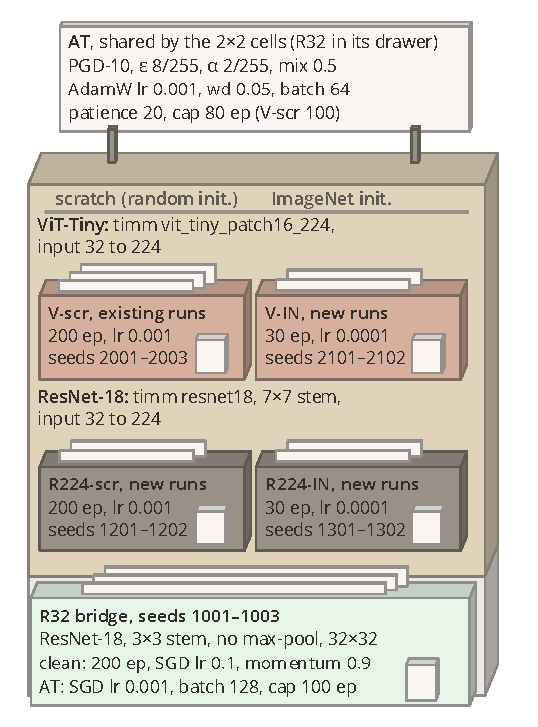
\includegraphics{fig2_design_recipe}
\caption{\textbf{Architecture-by-initialization design as a card cabinet.} On CIFAR-10 the drawer rows ViT-Tiny and ResNet-18 cross the columns scratch (random init.) and ImageNet init.; each drawer gives its clean stage (epochs, learning rate) and seeds, one index card per run. The R32 bridge drawer keeps its own recipe; the sign on top is the AT recipe of the four cells.}
\label{fig:fig2_design_recipe}
\end{figure}
